\documentclass[11pt]{article}
\usepackage[a4paper,left=1.5cm,right=1.5cm,top=1.5cm,bottom=1.5cm]{geometry}
\usepackage{fancyhdr}
\renewcommand{\headrulewidth}{1pt}
\fancyhead[C]{\textbf{[LINMA1170] Solveurs directs}}
\fancyhead[L]{Décembre 2018}
\fancyhead[R]{Gilles Peiffer [24321600]}

\usepackage[T1]{fontenc}
\usepackage[utf8]{inputenc}
\usepackage[french]{babel}
\usepackage{graphicx}
\usepackage{subcaption}
\usepackage{csquotes}
\usepackage{mathtools,amssymb}
\usepackage[binary-units=true,separate-uncertainty = true,multi-part-units=single]{siunitx}
\usepackage{float}
\usepackage[linktoc=all]{hyperref}
\hypersetup{breaklinks=true}
\setlength{\parskip}{1ex plus 0.5ex minus 0.2ex}
\newcommand{\hsp}{\hspace{20pt}}
\newcommand{\HRule}{\rule{\linewidth}{0.5mm}}
\graphicspath{{img/}}
\usepackage{caption}
\usepackage{textcomp}
\usepackage{array}
\usepackage{color}
\usepackage{tabularx,booktabs}
\usepackage{titlesec}
\titlespacing{\section}{0pt}{\parskip}{-\parskip}
\titlespacing{\subsection}{0pt}{\parskip}{-\parskip}
\titlespacing{\subsubsection}{0pt}{\parskip}{-\parskip}
\pagestyle{fancy}
\DeclarePairedDelimiterX{\norm}[1]{\lVert}{\rVert}{#1}
\usepackage{listings}
\lstset{
	language=Python,
	numbers=left,
	numberstyle=\tiny\color{gray},
	basicstyle=\rm\small\ttfamily,
	keywordstyle=\bfseries\color{dkred},
	frame=single,
	commentstyle=\color{gray}=small,
	stringstyle=\color{dkgreen},
	%backgroundcolor=\color{gray!10},
	%tabsize=8, % Thank you Papa Torvalds
	%rulecolor=\color{black!30},
	%title=\lstname,
	breaklines=true,
	framextopmargin=2pt,
	framexbottommargin=2pt,
	extendedchars=true,
	inputencoding=utf8,
}
\DeclareMathOperator{\dens}{\mathrm{dens}}

\begin{document}
\section*{Introduction}
Pour ce devoir, il était demandé d'écrire des fonctions en langage Python permettant de résoudre éfficacement un système d'équations linéaires issu d'un modèle d'éléments appelé \lstinline[language=bash]{ccore}.
Le devoir se divise en deux tâches:
\begin{itemize}
	\item la résolution d'un système en format plein et
	\item la résolution d'un système en format creux.
\end{itemize}
Pour la première partie, deux fonctions ont dû être écrites:
\begin{itemize}
	\item \lstinline|LUfactorize|, qui factorise en place la matrice $A \in \mathbb{C}^{n \times n}$ et
	\item \lstinline|LUsolve|, qui résout un système linéaire $Ax = b$.
\end{itemize}
La seconde partie fait la même chose pour une matrice dite \foreignquote{french}{creuse}.
Une heuristique de renumérotation est également implémentée pour profiter le plus possible de l'aspect creux de la matrice.

\section{Format plein}
\label{sec:dense}
Dans la partie en format plein du devoir, le but était d'étudier la densité de la factorisation \textsc{lu} en place d'une matrice de faible densité.
Pour faire cela, il a fallu écrire une fonction capable de faire cette factorisation: \lstinline|LUfactorize|.
Elle prend en arguments la matrice $A$ et décompose celle-ci en un produit d'une triangulaire supérieure $U$ et d'une matrice triangulaire inférieure à diagonale unité $L$ de sorte à ce que $A = LU$.

Pour résoudre le système, il suffit alors de d'abord calculer $Ly = b$ par substitution avant, puis de résoudre $Ux = y$ par substitution arrière pour trouver la solution $x$.
La fonction \lstinline|LUsolve| fait ceci.
\subsection{Étude de la densité de la décomposition \textsc{lu}}
\label{sec:fulldens}
Comme la matrice $A$ est issue d'un modèle d'éléments finis, elle contient beaucoup d'entrées nulles.
La densité d'une matrice est définie comme
\[
\dens A  = \frac{\textnormal{nnz}}{n^2}\,, \quad A \in \mathbb{C}^{n \times n}\,,
\]
où $\textnormal{nnz}$ est défini comme le nombre d'éléments non nuls de $A$.

Afin de faire une étude correcte de l'évolution de la densité de la matrice $A$ après sa décomposition \textsc{lu} en place, plusieurs graphes ont été réalisés.
Ils sont représentés à la Figure~\ref{fig:full_density}.
\begin{figure}[H]
	\centering
	\begin{subfigure}[t]{0.32\textwidth}
		\centering
		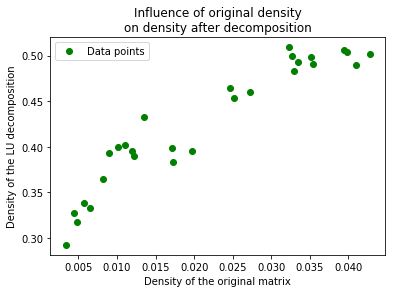
\includegraphics[width=\linewidth]{dens_adens_lu.png}
		\caption{Valeur de la densité après factorisation en fonction de la densité originelle.}
		\label{fig:a_dens__lu_dens}
	\end{subfigure}\hfill
	\begin{subfigure}[t]{0.32\textwidth}
		\centering
		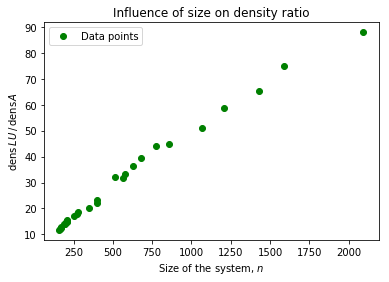
\includegraphics[width=\linewidth]{dens_ratio.png}
		\caption{Évolution du rapport entre la densité de la factorisation en place et la densité de la matrice originelle en fonction de la taille du système.}
		\label{fig:dens_ratio}
	\end{subfigure}\hfill
	\begin{subfigure}[t]{0.32\textwidth}
		\centering
		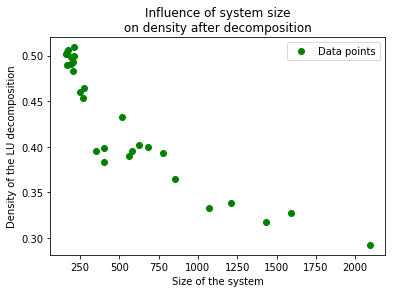
\includegraphics[width=\linewidth]{dens_lu__size.png}
		\caption{Influence de la taille du système sur la densité de la matrice après factorisation en place.}
		\label{fig:dens_lu__size}
	\end{subfigure}
	\caption{Différents graphes pertinents pour l'analyse de la section~\ref{sec:fulldens}.}
	\label{fig:full_density}
\end{figure}
On remarque que plus la matrice devient grande, plus elle devient creuse; c'est une propriété du modèle d'éléments finis. Sur le graphe de la Figure~\ref{fig:a_dens__lu_dens} , on remarque que la densité de la factorisation augmente lorsque la densité de $A$ augmente. Cependant, comme expliqué à la section~\ref{sec:rcmk}, ceci n'est qu'un rapport qualitatif.

En combinant le fait que la densité de $A$ diminue plus le système devient grand, et que la densité de la factorisation diminue lorsque la densité de $A$ devient plus petite, on peut prédire par transitivité que plus le système devient grand, plus la densité de sa factorisation LU va diminuer.
C'est ce qu'on observe sur le graphe de la Figure~\ref{fig:dens_lu__size}.
Finalement, le rapport de la densité de la matrice après factorisation sur sa densité avant factorisation est représenté comme une fonction de la taille du système à la Figure~\ref{fig:dens_ratio}.

\subsection{Complexité temporelle de \texttt{LUsolve}}
Le solveur \lstinline|LUsolve| fait trois choses séquentiellement, et la complexité totale est donc la somme des trois complexités partielles.
\subsubsection{Complexité temporelle de \texttt{LUfactorize}}
Il s'agit ici de calculer le nombre d'opérations pour une décomposition \textsc{lu} en place. Pour cela, on se réfère au livre de référence p.151.
Le nombre d'opérations de l'Algorithme~20.1 est dominé par l'opération vectorielle $u_{j, k:n} = u_{j, k:n} - \ell_{jk} u_{k, k:n}$.
On voit que celle-ci effectue une multiplication scalaire-vecteur et une soustraction entre vecteurs.
Soit $l = n - k - 1$ la longueur des vecteurs-lignes étant manipulés. Le nombre de \emph{flops} est alors de $2l$.
Pour chaque valeur de $k$, l'indice de la boucle extérieure, la boucle intérieure est répétée pour toutes les lignes de $k+1$ jusque $n$.
La complexité de \lstinline|LUfactorize|, $d(n)$, est alors
\[
d(n) \sim \sum_{k=1}^{n} 2 (n - k) (n - k + 1) = 2 \sum_{j=0}^{n-1} j (j+1) = 2 \sum_{j=0}^{n-1} j^2  + 2 \sum_{j=0}^{n-1} j = \frac{2 n^3}{3} - n^2 + \frac{n}{3} + n^2 - n \sim \frac{2 n^3}{3}\,. 
\]
\subsubsection{Complexité temporelle de la substitution arrière}
La complexité temporelle de la substitution arrière, $b(n)$, est due à $\frac{n^2 - n}{2}$ soustractions, $\frac{n^2 - n}{2}$ multiplications et $n$ divisions. Le calcul complet est
\[
b(n) \sim \sum_{j=1}^{n} \big(2(n - j) + 1 \big) \sim 2 \sum_{k=0}^{n-1} k + n = n (n - 1) + n = n^2\,.
\]

\subsubsection{Complexité temporelle de la substitution avant}
Comme pour la substitution arrière, la complexité temporelle pour la substitution avant, $f(n)$, est due à $\frac{n^2 - n}{2}$ soustractions et $\frac{n^2 - n}{2}$ multiplications.
Le calcul complet est alors
\[
f(n) \sim \sum_{j=1}^{n} 2(n-j) = 2 \sum_{k=0}^{n-1} k = n (n-1) \sim n^2\,.
\]

\subsubsection{Complexité totale}
Comme dit plus haut, pour trouver $s(n)$, la complexité temporelle totale, il suffit de sommer les 3 complexités (comme les opérations se font en série).
On trouve alors
\[
s(n) = d(n) + b(n) + f(n) \sim \frac{2n^3}{3} + n^2 + n^2 \sim \frac{2n^3}{3}\,.
\]
Comme on peut le voir, l'étape de factorisation est dominante pour la complexité temporelle. On voit sur le graphe de la Figure~\ref{fig:lusolve_time} que cette prédiction théorique est confirmée expérimentalement. Mentionnons finalement que comme les matrices sont issues d'un modèle d'éléments finis, elles sont symétriques (hermitiennes) et définies positives; il n'est alors pas nécessaire de rajouter une vérification pour éviter les divisions par zéro dans \lstinline|LUfactorize|. Ceci peut se démontrer par le critère de Sylvester.
\begin{figure}[H]
	\centering
	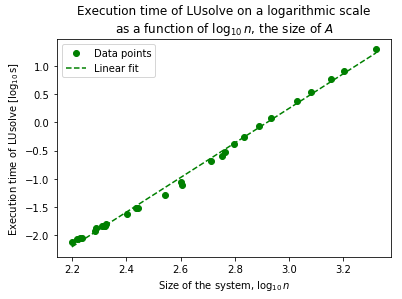
\includegraphics[width=0.37\textwidth]{lusolve_time.png}
	\caption{Temps d'exécution de la fonction \lstinline|LUsolve| en fonction de la taille du système, en échelle logarithmique.}
	\label{fig:lusolve_time}
\end{figure}

\section{Format creux}
Comme expliqué dans l'introduction, les matrices issues de \lstinline[language=bash]|ccore| sont très creuses.
Il serait donc intéressant de trouver une manière de résoudre le système sans avoir à faire autant de calculs. Pour cela, il serait utile d'avoir une représentation de la matrice qui n'utilises pas autant de mémoire.
Pour faire cela, nous utilisons le format \textsc{csr} et la fonction \lstinline|CSRformat|.
Une fois cette représentation obtenue, il est possible d'améliorer la complexité de la résolution du système par factorisation \textsc{lu}.
Comme expliqué à la section~\ref{sec:LUcsrsolve}, cette complexité va dépendre de la largeur de bande de la matrice $A$.
La section~\ref{sec:rcmk} détaille comment profiter plus de cette nouvelle complexité.
\subsection{Performances de \texttt{CSRformat}}
\label{sec:csrformat}
La fonction \lstinline|CSRformat| parcourt toute la matrice, ligne par ligne, en copiant toutes les entrées non nulles dans un vecteur \lstinline|sA|, leurs indices de colonne dans \lstinline|jA| et l'indice de leur premier élément non nul dans \lstinline|iA|.
On voit donc facilement que cette fonction doit avoir une complexité temporelle de $\Theta(n^2)$. Les opérations les plus coûteuses effectuées sont:
\begin{itemize}
	\item parcours de la matrice pour trouver la valeur de $\textnormal{nnz}$ en $\Theta(n^2)$;
	\item $n$ recherches d'indices et de valeurs d'éléments non nuls en $\Theta(n^2)$ au total;
\end{itemize}
On voit donc bien que la complexité totale est également en $\Theta(n^2)$, ce qui se voit sur le graphe de la Figure~\ref{fig:csrformat}.
\begin{figure}[H]
	\centering
	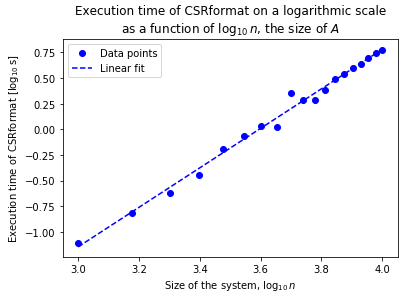
\includegraphics[width=0.37\textwidth]{csrformat.png}
	\caption{Temps d'exécution de la fonction \lstinline|CSRformat| en fonction de la taille du système, en échelle logarithmique.}
	\label{fig:csrformat}
\end{figure}
\subsection{Complexité temporelle de \texttt{LUcsrsolve}}
\label{sec:LUcsrsolve}
La fonction \lstinline|LUcsrsolve| est une version optimisée de \lstinline|LUsolve| spécifiquement pour les matrices creuses.
Définissons la largeur de bande $k$ de $A$ comme étant
\[
k = \max(k_1, k_2)\,, \quad \textnormal{où} \quad a_{ij} = 0 \quad \textnormal{si} \quad j < i - k_1 \quad \textnormal{ou} \quad j > i + k_2\,; \quad k_1, k_2 \ge 0\,.
\]
En effet, une des propriétés de la factorisation \textsc{lu} est que lors de la décomposition, des nouvelles entrées non nulles peuvent apparaître mais uniquement à l'intérieur de la bande de la matrice (phénomène de \emph{fill-in}). On peut donc préallouer facilement cette bande, la remplir au fur et à mesure de la factorisation, et n'avoir qu'à considérer une partie de cette bande (et donc de la matrice $A$) lors des substitutions.

Pour calculer la complexité de la fonction \lstinline|LUcsrsolve|, il faut observer qu'elle sera égale à la somme des complexités de \lstinline|CSRformat| ($\Theta(n^2)$, voir section~\ref{sec:csrformat}), \lstinline|LUcsr|, et de deux substitutions modifiées.
\subsubsection{Complexité temporelle de \texttt{LUcsr}}
La fonction \lstinline|LUcsr| a une complexité qui dépend de plusieurs étapes:
\begin{itemize}
	\item calcul de la largeur de bande en $\Theta(n)$ grâce au format \textsc{csr};
	\item préallocation de vecteurs en $\mathcal{O}(nk)$;
	\item décomposition \textsc{lu} creuse en $\mathcal{O}(nk^2)$.
\end{itemize}
Pour trouver $\lambda(n, k)$, la complexité de la décomposition \textsc{lu} creuse, on observe que la boucle intérieure fait une multiplication et une soustraction, et on calcule (en idéalisant un peu)
\[
\lambda(n, k) \in \mathcal{O}\bigg(\sum_{i=0}^{n-1}\ \  \sum_{j = i+1}^{\min(i+k_1+1, n)} \ \ \sum_{m = i+1}^{\min(i+k_2+1, n)} 2\bigg) \in \mathcal{O}\bigg(2 \sum_{i=0}^{n-1} k_1 k_2\bigg) \in  \mathcal{O}(n k^2)\,.
\]
Cette complexité-ci domine le temps d'exécution de \lstinline|LUcsr|.
\subsubsection{Complexité des substitutions modifiées}
Dans les substitutions modifiées, on peut utiliser le fait que seule la partie non nulle de la matrice nous intéresse. On écrit alors la complexité $\sigma(n, k)$ des deux substitutions en série comme
\[
\sigma(n, k) \sim \sum_{i=0}^{n} k_1 + \sum_{i=0}^{n} k_2 \sim 2nk\,.
\]
\subsubsection{Complexité totale de \texttt{LUcsrsolve}}
Comme dit plus haut, ces opérations se font toutes en série, et la complexité totale $t(n, k)$ s'écrit alors
\[
t(n, k) \in \mathcal{O}(n^2 + nk^2 + nk) \in \mathcal{O}(nk^2)\,.
\]
La factorisation est donc l'étape contribuant le plus à la complexité temporelle.
\subsection{Numérotation \foreignquote{french}{reverse Cuthill-McKee}}
\label{sec:rcmk}
Comme expliqué à la section~\ref{sec:LUcsrsolve}, la complexité de la fonction \lstinline|LUcsrsolve| dépend du carré de la largeur de bande.
Il serait donc intéressant d'utiliser un algorithme de renumérotation des n\oe{}uds tel que \textsc{rcmk} pour diminuer cette largeur de bande.

Cet algorithme n'influence pas uniquement la complexité en temps mais aussi en mémoire: lors du \emph{fill-in} de la décomposition \textsc{lu}, plus la bande est petite, plus on peut borner la densité de la matrice résultant de la factorisation en place.

\begin{figure}[H]
	\centering
	\begin{subfigure}[t]{0.27\textwidth}
		\centering
		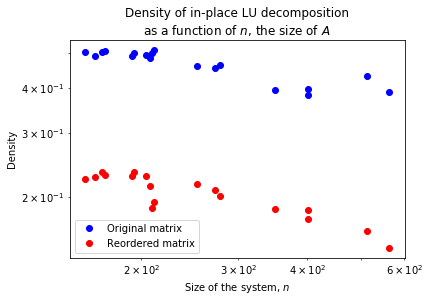
\includegraphics[width=\linewidth]{rcmk_dens.png}
		\caption{Comparaison entre la densité de la factorisation avec et sans \textsc{rcmk}.}
		\label{fig:rcmk_dens}
	\end{subfigure}\hfill
	\begin{subfigure}[t]{0.27\textwidth}
		\centering
		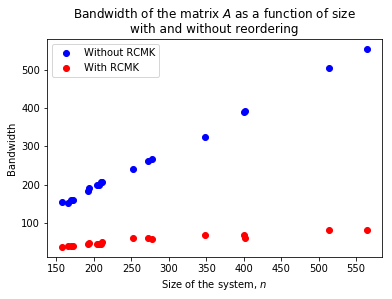
\includegraphics[width=\linewidth]{bandwidth.png}
		\caption{Influence de \textsc{rcmk} sur la largeur de bande de $A$.}
		\label{fig:bandwidth}
	\end{subfigure}\hfill
	\begin{subfigure}[t]{0.2\textwidth}
		\centering
		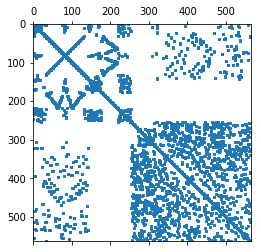
\includegraphics[width=\linewidth]{spy.png}
		\caption{Matrice $A$ sans renumérotation \textsc{rcmk}.}
		\label{fig:spy}
	\end{subfigure}\hfill
	\begin{subfigure}[t]{0.2\textwidth}
		\centering
		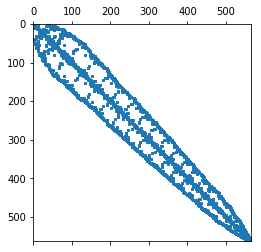
\includegraphics[width=\linewidth]{spy_rcmk.png}
		\caption{Matrice $A$ avec renumérotation \textsc{rcmk}.}
		\label{fig:spy_rcmk}
	\end{subfigure}
	\caption{Influence de la renumérotation \textsc{rcmk} sur la densité de $A$.}
	\label{fig:rcmk}
\end{figure}
Sur la Figure~\ref{fig:rcmk}, on peut voir que la densité de la factorisation \textsc{lu} diminue lorsque la matrice est permutée (Figure~\ref{fig:rcmk_dens}) et que la largeur de bande de la matrice $A$ diminue (et augmente beaucoup moins rapidement) lorsque la matrice est permutée (Figure~\ref{fig:bandwidth}).

\subsection{Complexité de \texttt{LUcsrsolve} avec renumérotation \textsc{rcmk}}
Afin d'évaluer l'utilité de cette renumérotation, il est utile de regarder l'évolution de la complexité lorsqu'on applique la permutation. Il faut alors rajouter deux étapes à la fonction: le calcul de la permutation optimale (fonction \lstinline|RCMK|) et son application.
\subsubsection{Complexité du calcul de la permutation}
L'étape dominante pour la complexité temporelle est le fait de devoir trier à chaque itération la liste des n\oe{}ds adjacents au n\oe{}ud venant de sortir de la file. Or, nous pouvons borner la taille de cette liste de n\oe{}uds adjacents par le degré maximal dans le graphe, $\Delta(G) \le k_1+k_2 \le 2k$. En assumant qu'un algorithme de tri avec une complexité dans le pire cas inéarithmique, tel que \emph{mergesort}, soit utilisé, on peut alors dire que la fonction \lstinline|RCMK| appliquée au graphe $G(E, V)$ dont $A$ est la matrice d'adjacence a une complexité $r(G)$en $\mathcal{O}(|V(G)| \Delta(G) \log \Delta(G)$, ou avec les paramètres de notre système $n$ et $k$, 
\[
r(n, k) \in \mathcal{O}(n (2k) \log(2k) \in \mathcal{O}(nk \log k)\,.
\]
\subsubsection{Complexité de l'application de la permutation}
Pour permuter la matrice, on peut imaginer qu'il faut permuter d'abord les lignes puis les colonnes. Pour les lignes, il faut donc déplacer au plus $2nk$ éléments (comme une ligne a au plus de l'ordre de $2k$ entrées), et pour les colonnes la même chose.
Il est alors possible d'appliquer la permutation en $\mathcal{O}(nk)$.
\subsubsection{Complexité de \texttt{LUcsrsolve} avec renumérotation \textsc{rcmk}}
La complexité totale $\tau(n, k)$ pour \lstinline|LUcsrsolve| avec renumération est alors
\[
\tau(n, k) \in \mathcal{O}(nk^2 + nk \log k + nk) \in \mathcal{O}(nk^2)\,,\quad \textnormal{car} \quad \lim_{(n, k) \to (+\infty, +\infty)} (nk^2 + nk \log k) = \lim_{(n, k) \to (+\infty, +\infty)} nk^2\,.
\]
C'est la même complexité que pour \lstinline|LUcsrsolve| sans renumérotation, mais on remarque que comme la largeur de bande a fortement diminué, la résolution du système sera beaucoup plus rapide pour les matrices creuses.
C'est aussi ce qu'on observe sur la Figure~\ref{fig:all_exec_time}.
Le temps d'exécution de la fonction \lstinline|RCMK| est montré sur la Figure~\ref{fig:rcmk_exec}.
On observe que le solveur plein est plus rapide pour les matrices de ces tailles (grâce à la vectorisation et aux opérations optimisées de \lstinline[language=bash]|BLAS|), mais la pente pour le solveur avec \textsc{RCMK} est plus petite, et asymptotiquement, cette méthode sera plus rapide.
\begin{figure}[H]
	\centering
	\begin{subfigure}[t]{0.37\textwidth}
		\centering
		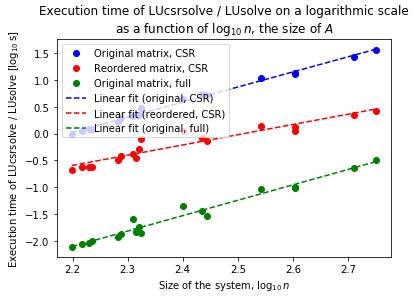
\includegraphics[width=\linewidth]{all_exec_time.png}
		\caption{Temps d'exécution pour les différents solveurs.}
		\label{fig:all_exec_time}
	\end{subfigure}%
	\begin{subfigure}[t]{0.37\textwidth}
		\centering
		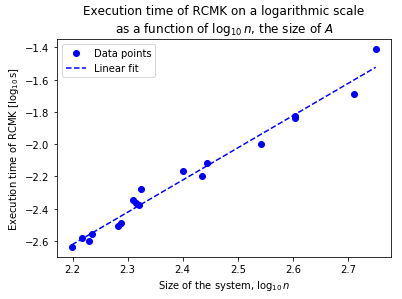
\includegraphics[width=\linewidth]{rcmk_exec.png}
		\caption{Temps d'exécution pour le calcul de la permutation \textsc{rcmk}.}
		\label{fig:rcmk_exec}
	\end{subfigure}
	\caption{Influence de la renumérotation \textsc{rcmk} sur le temps d'exécution du solveur.}
	\label{fig:rcmk_solve}
\end{figure}
Un autre point intéressant est que dans le cas de matrices très mal numérotées ($k = n$), l'algorithme creux devient un simple algorithme de factorisation en $\mathcal{O}(n^3)$ et sa pente est égale à la pente pour le solveur plein.

Afin d'évaluer la complexité du solveur creux dans le cas d'une renumérotation \textsc{rcmk}, voici un tableau avec des valeurs.

\end{document}